\documentclass[conference]{IEEEtran}
\usepackage{fancyhdr}
\usepackage{multirow}
\usepackage{amsmath}
\usepackage{graphicx}
\usepackage{cite}
\usepackage{amsfonts}
\usepackage{listings}
\usepackage[colorlinks=true,
            urlcolor  = blue,
            citecolor = red]{hyperref}

\lstset{language=Python}
\setlength{\headheight}{15.2pt}
\pagestyle{fancy}
\renewcommand{\headrulewidth}{0pt} % no line in header area
\fancyhead{}
\lhead{Mini-Project \#3}
\chead{Handwritten Digits Classification}
\rhead{COMP 598}
\fancyfoot{}


\author{David Rapoport, Zafarali Ahmed, Pascale Gourdeau\\Team Name: TBD}
\title{COMP-598 Mini-Project \#3\\Handwritten Digits Classification}
\date{\today}
\begin{document}
\maketitle

\section{Introduction}
The MNIST database\cite{MnistHome} of handwritten digits is often used as a baseline to compare performance of different classifiers. In this paper, we use a modified version of the MNIST database where the digits have been modified by (1) embossing, (2) rotation, (3) rescaling, and (4) random texturing. This makes the problem much more difficult and we demonstrate poor performance with linear classifiers.

In this work we explore the performance of three classifiers: (1) Logistic Regression, (2) Support Vector Machine and (3) The Feed-forward Neural Network. 

<Something about results>

We then explore two algorithms, the tried and tested Convolution Neural Network \cite{LeCunn98}\cite{CNN_committees} and the brand new Spatial Transformer Network \cite{STN} to find that ......


\section{Related Work}




\section{Data}
The dataset was obtained from the Kaggle Competition Website. It is a modification of the MNIST \cite{MnistHome} database. A sampling of some digits can be seen in Fig \ref{MNISTSample} and it is apparent that this proves to be a difficult task for even humans to distinguish. In particular, we expect the digits $6$ and $9$ to be almost indistinguishable.

\begin{figure}[h]
	\centering
	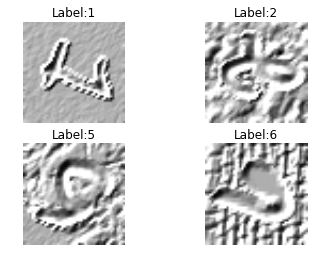
\includegraphics[scale=0.40]{sample_of_images.png}
	\caption{A sampling of the modified MNIST database}
	\label{MNISTSample}
\end{figure}

\section{Methodology}

We used the \href{http://www.numpy.org/}{NumPy package} and the \href{http://www.scikit-learn.org/}{scikit-learn library} to perform feature extraction and selection, implement our classifiers, and analyse our results. 

\subsection{Feature Extraction and Preprocessing}


\subsection{Feature Selection}

We explored both Principal Component Analysis (PCA) and scaling the data as methods of dimensionality reduction and feature preprocessing. Principal Component analysis is a dimensionality reduction technique which tries to find a pair of linear transformations $f:\mathbb{R}^m\rightarrow\mathbb{R}^p$ and $g:\mathbb{R}^p\rightarrow\mathbb{R}^m$ where $p\leq m$ and for the corresponding matrices $F=G^T$. To find these matrices we are going to solve the equation $argmin_{F,G}\Sigma_{i=0}^N\|x_i-G\times F\times x_i\|^2$. Practically, we used scikit-learn's Incremental PCA which performs PCA in steps to avoid a memory blow up. 

\begin{figure}[Feature preprocessing grid search]
	\centering
	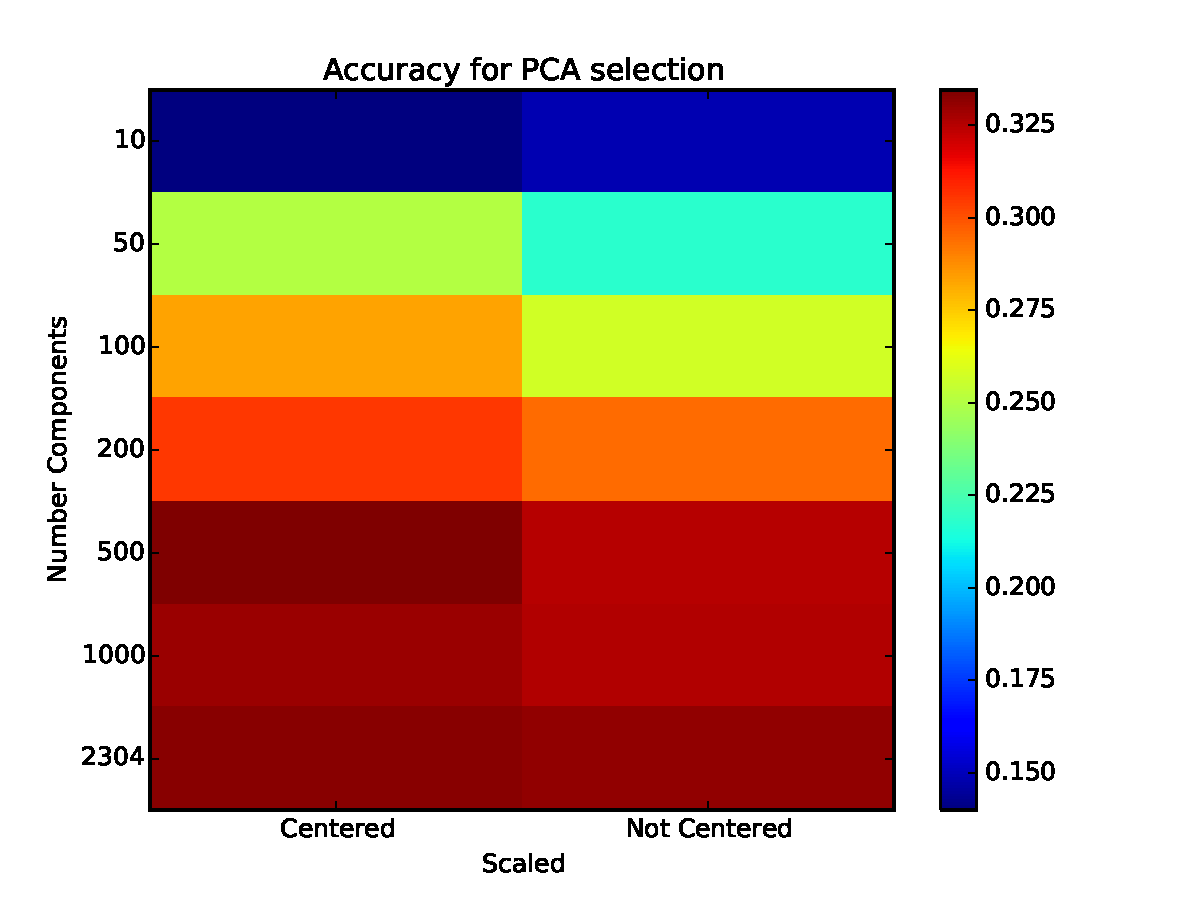
\includegraphics[scale=0.40]{PCA_gridsearch.pdf}
	\caption{The effect of varying the number of components and scaling the data}
	\label{gridsearchpca}
\end{figure}

We also scaled our data prior to use so that all features would have approximately zero mean and a standard deviation of roughly one. This was also done to more easily merge the modified digits dataset with the original MNIST dataset. Upon inspection we noticed that the original MNIST dataset took values of 0-255 while the modified MNIST dataset took values between 0-1, normalizing both datasets put them both on about the same scale. 

We performed a GridSearch on different values of p to use as the projected dimensionality of the data after applying PCA, and with and without scaling. \ref{gridsearchpca} shows the heatmap of our GridSearch using an SVM with an RBF kernel and C=10, gamma=1e-4, we get optimal results for p=500 and normalizing the data. 

\subsection{Generating Extra Data}

As per the suggestions of Patrice Simard et al. \cite{Simard} we decided to augment our learners with extra data. The data generated came from two different sources and the effect of the addition of either supplementary dataset is explored later in this paper.

\begin{figure}[Extra Data]
	\centering
	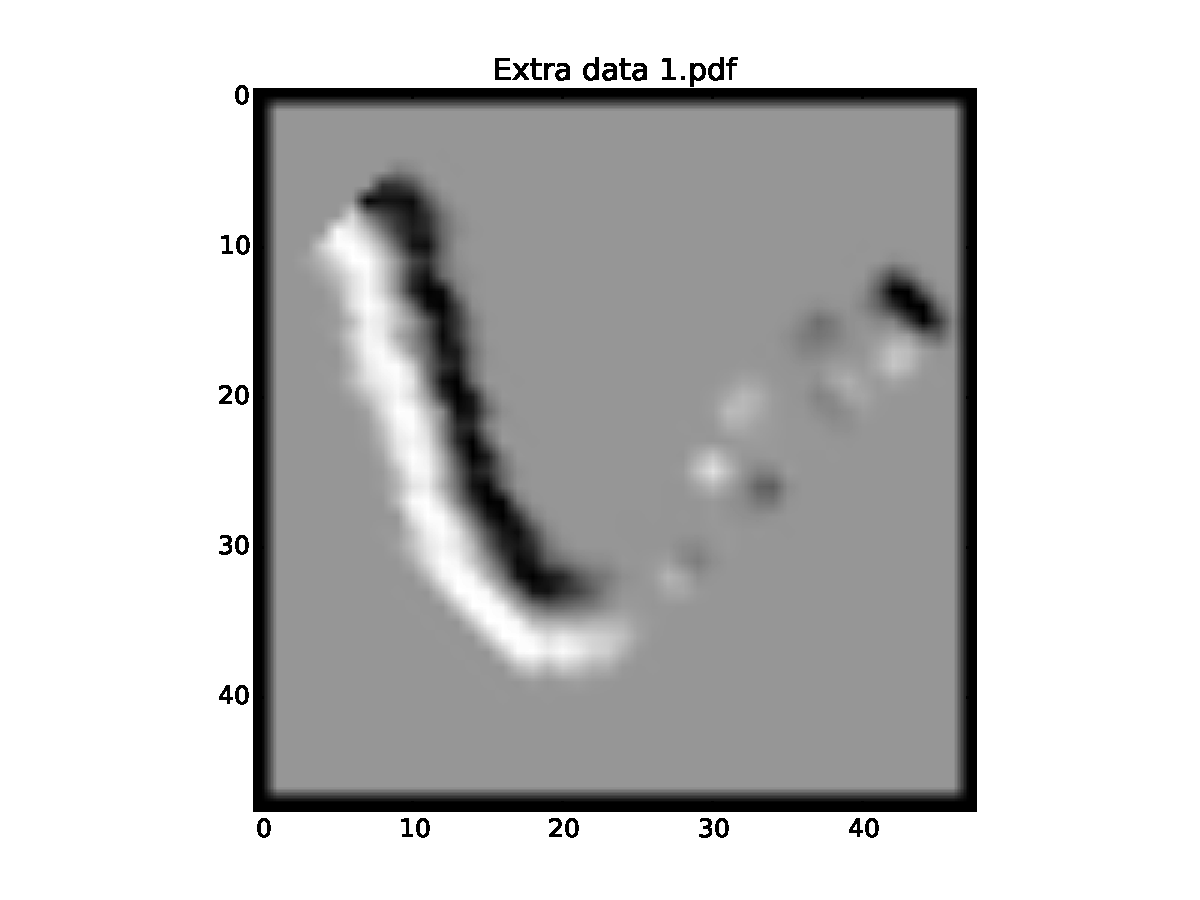
\includegraphics[scale=0.20]{Extradata1.pdf}
	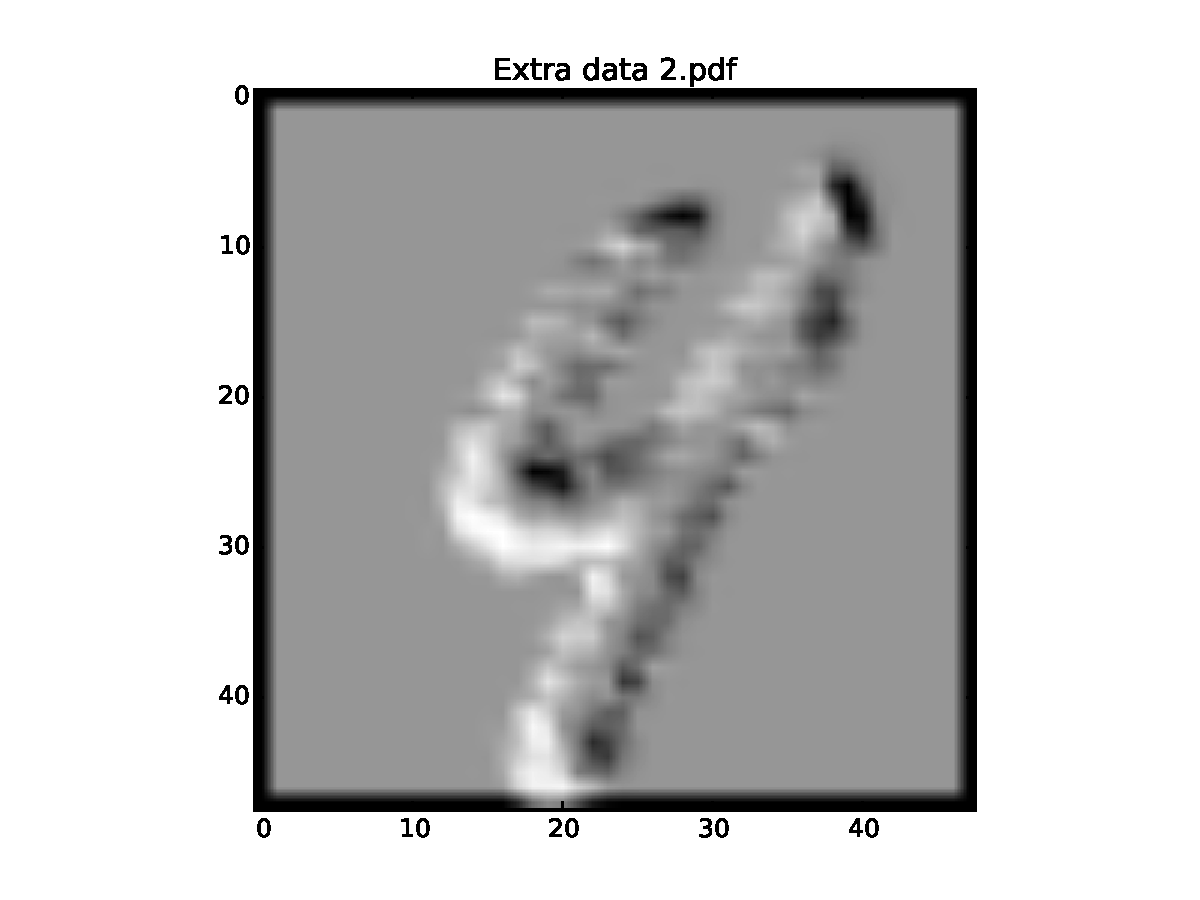
\includegraphics[scale=0.20]{Extradata2.pdf}
	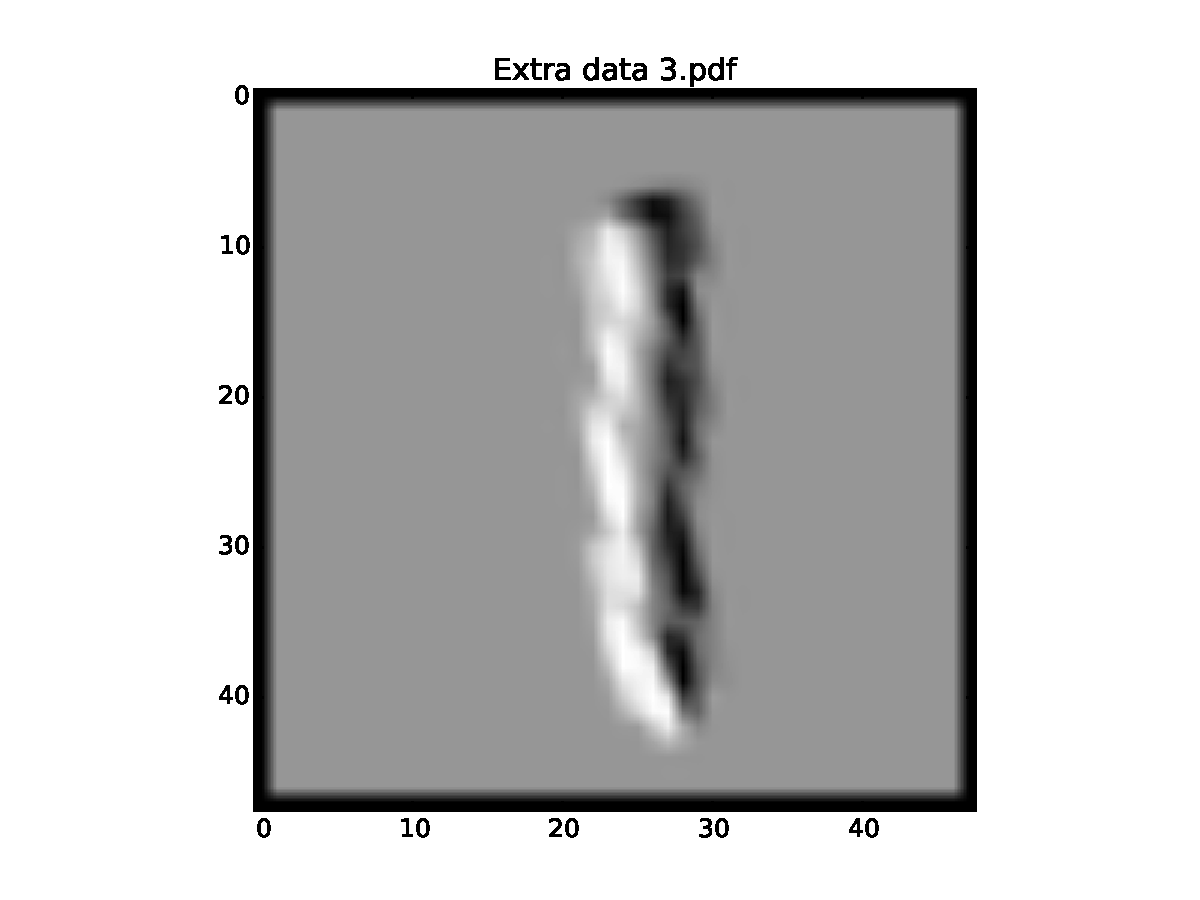
\includegraphics[scale=0.20]{Extradata3.pdf}
	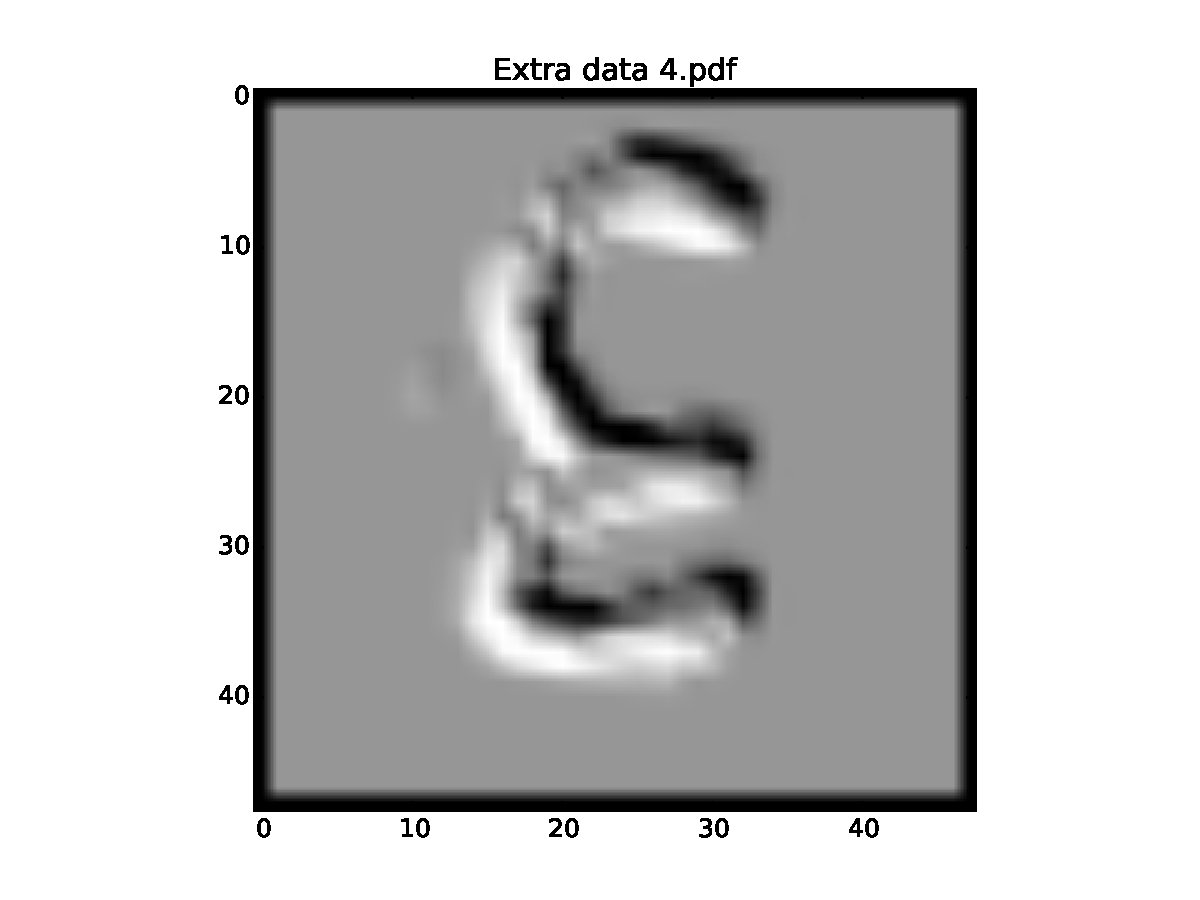
\includegraphics[scale=0.20]{Extradata4.pdf}
	\caption{Four example image from the "Extra Digits" dataset}
	\label{ExtraData}
\end{figure}

The first additional datasource involved transformations of the original MNIST dataset \cite{MNIST_Original}. We wil refer to this dataset as "Extra Digits" throughout the rest of the paper. First we enlarged the images from $28\times 28$ to $48\times 48$. Then we rotated by a random angle $\theta \in  [0,359]$. Finally we applied an emboss to the image. We attempted to add a pattern to the new image as in the modified MNIST dataset, but were unable to find a pattern which we felt maintained the integrity of the image in a way which the patterns used in the modified MNIST dataset did. An example of images from the dataset is shown in \ref{ExtraData}

\begin{figure}[Extra Data]
	\centering
	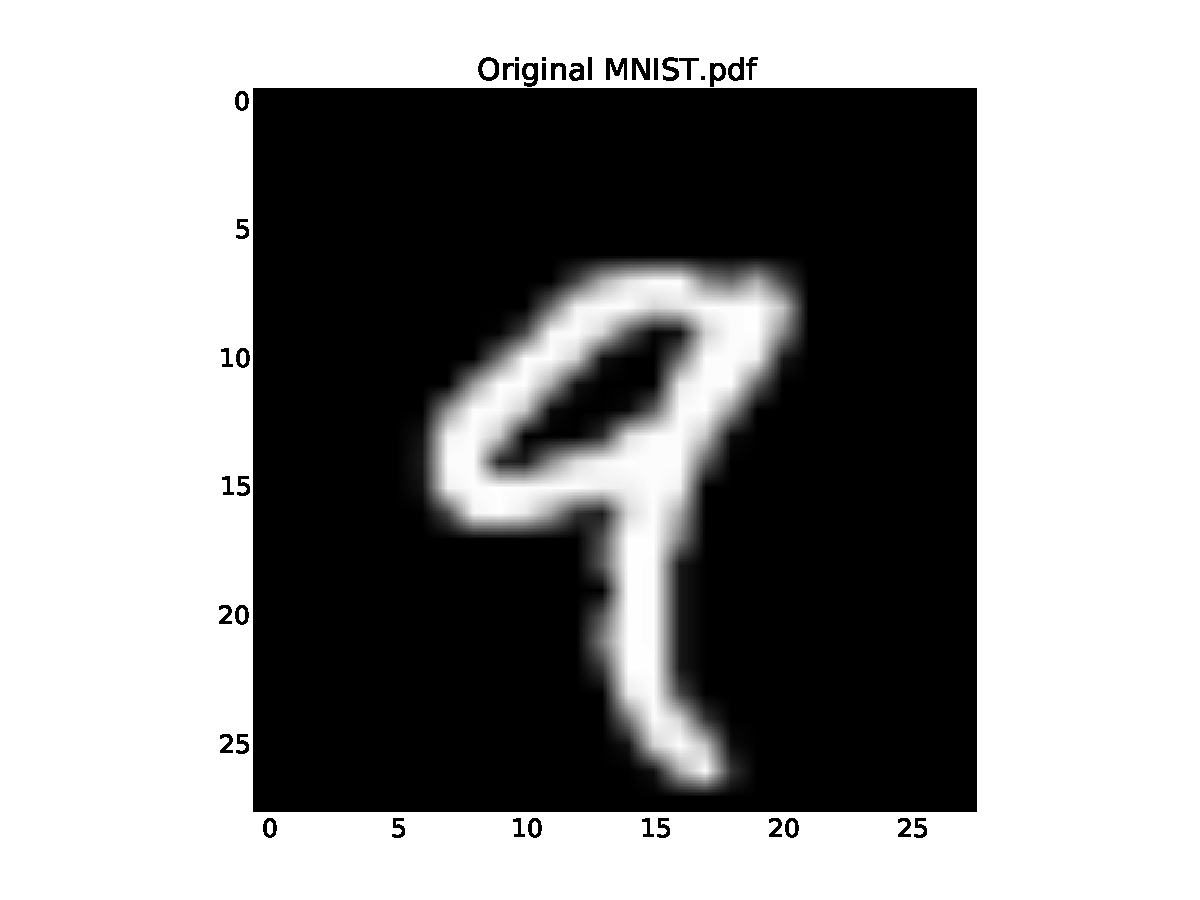
\includegraphics[scale=0.30]{OriginalMNIST.pdf}
	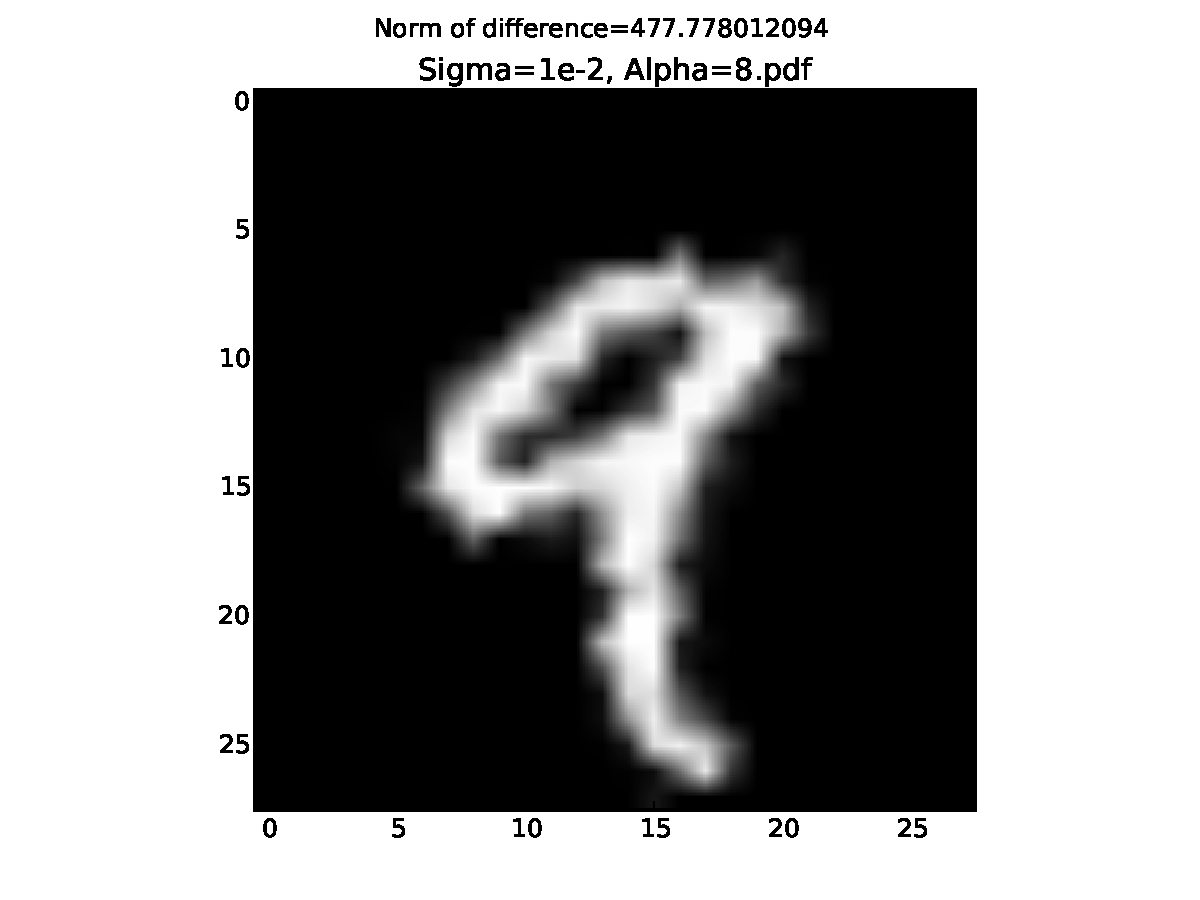
\includegraphics[scale=0.30]{Sigma=1e-2,Alpha=8.pdf}
	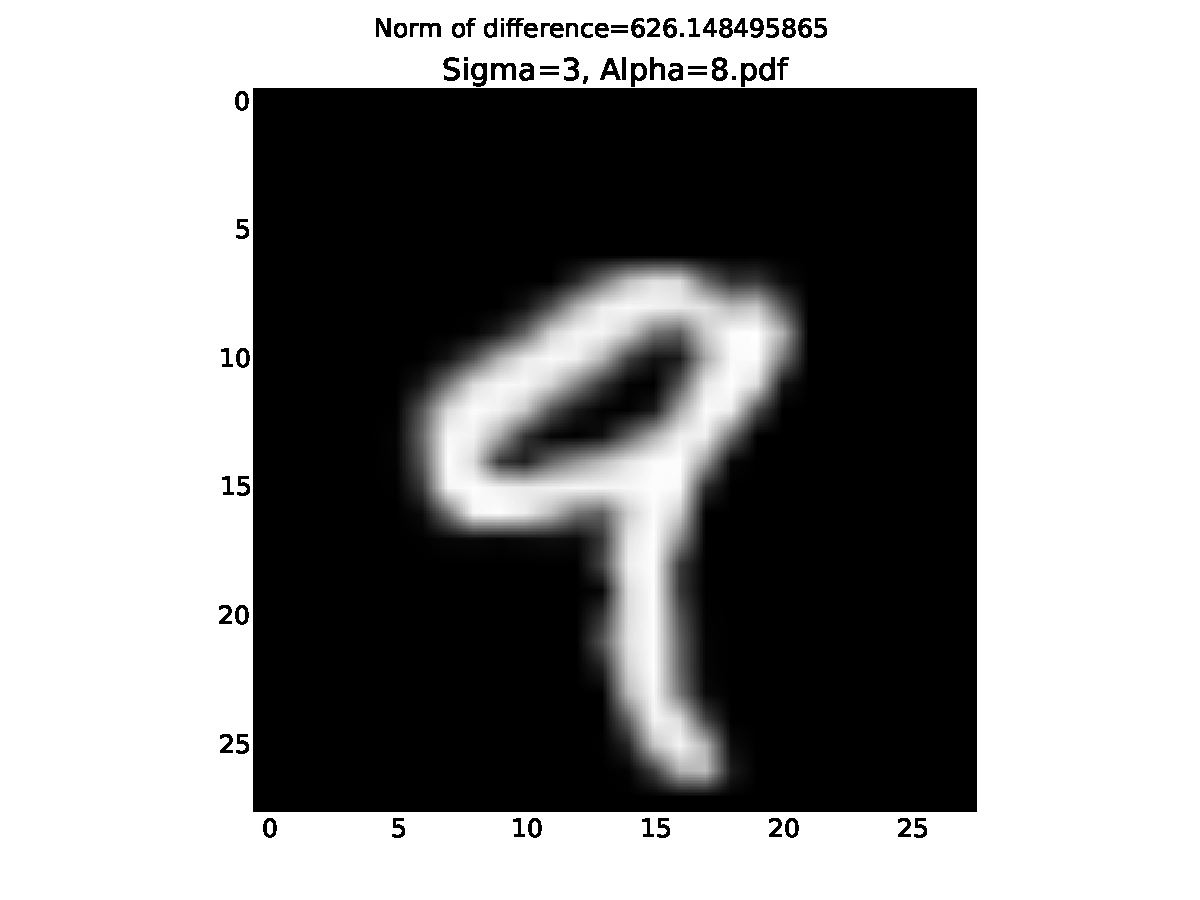
\includegraphics[scale=0.30]{Sigma=3,Alpha=8.pdf}
	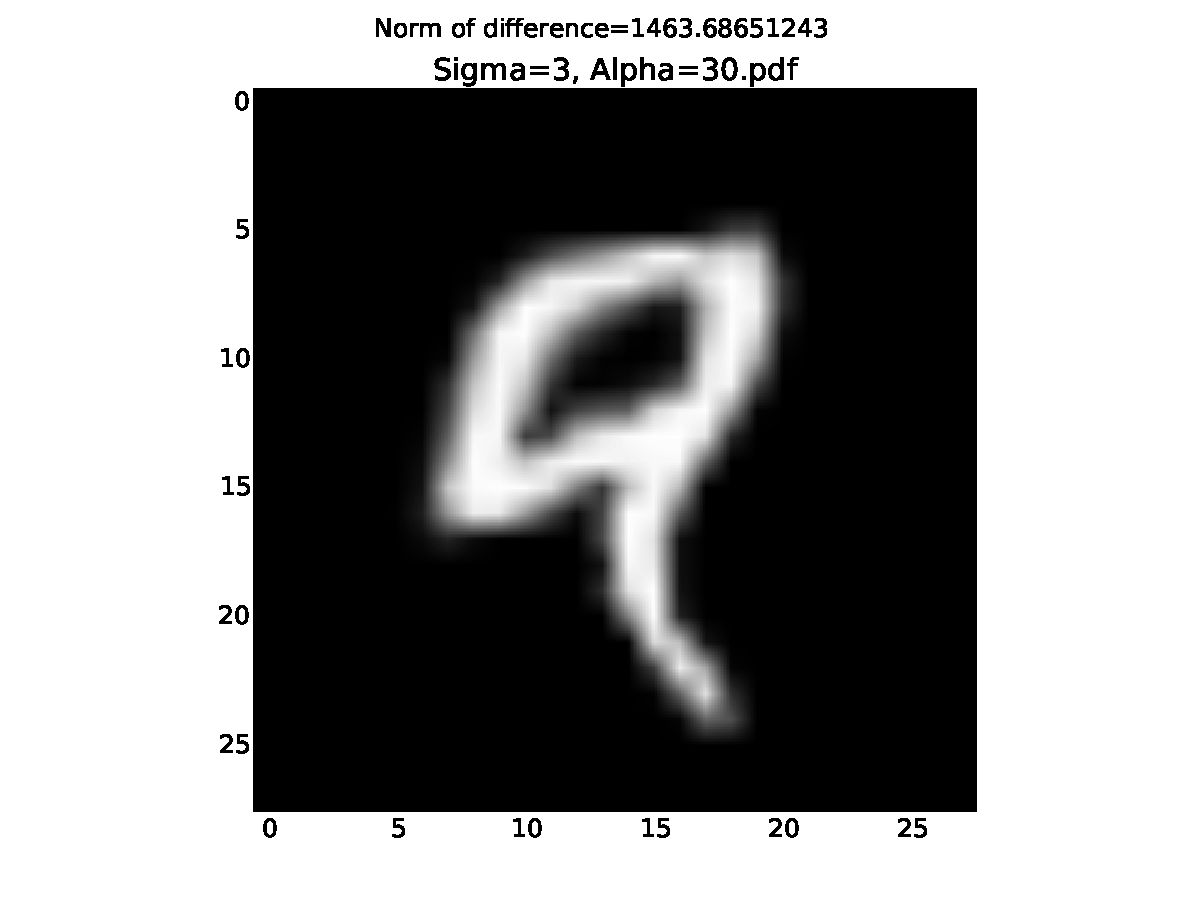
\includegraphics[scale=0.30]{Sigma=3,Alpha=30.pdf}
	\caption{The effect of varying $\sigma$ and $\alpha$}
	\label{Perturbed}
\end{figure}

The second datasource we attempted to generate was motivated by Patrice Simard et al. \cite{Simard}. This involved performing an affine deformation of the modified MNIST image. We refer to this additional dataset as "Perturbed Modified Digits" throughout the rest of the paper. The methodology for generating these perturbed digits is as follows. Given a $n\times n$ image, we first generate two random $n\times n$ displacement fields $?x(x',y')\rightarrow uniform(-1,1)$ and $?y(x',y')\rightarrow uniform(-1,1)$. We the convolve these displacement fields by a gaussian filter with $\mu = 0$ and $\sigma$ being a variable to the function which defaults to 3. After this we normalize the displacement fields by dividing each element in the field by the norm of the matrix. All the elements in both displacement fields are then multiplied by $\alpha$ which is a variable to the function. We then generate a new $n\times n$ image as such: for each pixel $(i,j)$ in the original, the new value at that pixel is the value at $?x(i,j),?y(i,j)$ in the original picture. Bilinear interpolation is used to determine the value of $new(i,j)=original(?x(i,j),?y(i,j))$ when $?x(i,j),?y(i,j)$ are not integers. For indices which appear out of bounds of the picture we simply used a default value of 0. \ref{Perturbed} shows the effect of varying $\alpha$ and $\sigma$ on the original MNIST dataset (similar results occur with the modified dataset, but are harder to distinguish). The norm of the difference between the original MNIST image and the modified image are included in the pictures. We found that increasing $\alpha$ causes larger smooth, deformations while decreasing $\sigma$ causes the deformation to be more random and noisy. This is consistent with the findings in the literature.

\begin{figure}[h]
	\centering
	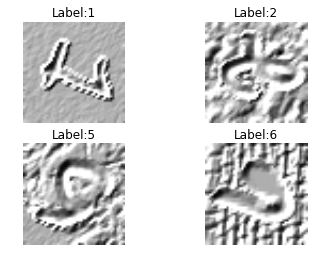
\includegraphics[scale=0.40]{sample_of_images.png}
	\caption{A sampling of the modified MNIST database}
	\label{MNISTSample}
\end{figure}

\subsection{Classification Algorithms}

\subsubsection{Baseline: Logistic Regression}
In Logistic Regression, we want to estimate the probability that some random vector $X=(x_1, \ldots, x_n)$ has a class $Y=y_k$, $P(Y=y_k | X=(x_1, \ldots, x_n))$. In the binary case we can derive the following using Bayes rule and conditioning:
\begin{equation*}
\begin{split}
&P(Y=1~|~X) = \frac{P(X, Y=1)}{P(X)}\\
&= \frac{ P(X~|~Y=1)\cdot P(Y=1) }{ P(X~|~Y=1)\cdot P(Y=1) + P(X~|~Y=0)\cdot P(Y=0) }\\
& = \frac{1}{1 + \exp{(-a)}} = \sigma(a) \text{~(Sigmoid Function)}\\
\end{split}
\end{equation*}

where $a=\ln\Big(\frac{P(Y=1~|~X)}{P(Y=0~|~X)}\Big)$ is the log-odds ratio. By approximating the log-odds ratio as a linear decision boundary of the features and weights, $w^T x$ we can use this as an estimate of the class being $Y=1$. We can optimize the Log-likelihood or Cross-Entropy function:

\begin{equation}
	\label{LL}
	L(w) = -\sum_{i=1}^n y_i\log\Big(\sigma(w^Tx_i)\Big) + (1-y_i)\log\Big(1-\sigma(w^Tx_i)\Big)
\end{equation}

and search for the optimal set of weights using the \emph{gradient descent algorithm} with $N$ steps and update rule \ref{LR_update_rule}:

\begin{equation}
\label{LR_update_rule}
	w_{k+1} = w_k + \alpha_k \sum_{i=1}^n \Big( x_i\big(y_i - \sigma(w_k^Tx_i\big) \Big)
\end{equation}


\subsubsection{SVM}
We selected our kernel through cross validation and we tested polynomial kernels of degree 2-9, linear kernel, and an RBF kernel. The results for this cross validation and others can be seen in the results section, but the best kernel was the RBF kernel. The RBF (Radial Basis Function) kernel is defined as such \cite{Hastie}: \[K(x,x\prime )=exp(-\gamma\|x-x\prime \|^2)\] It is evident that gamma is the parameter which sets the approximately the inverse radius of influence of any training example $x_i$. A low value of gamma means that an examples will have an influence on training examples far away from itself, while a large gamma means that an example has a very local area of influence \cite{sklearn}.

\subsubsection{Fully Connected Feedforward Neural Network}

\subsubsection{Convolution Neural Network}
The convolution neural network \ref{LeCunn98} is a neural network with specialized layers in which not all neurons are connected to each other. Infact the main component is the subblayer (Fig \ref{convmaxlayer}) which contains the Convolution2D and MaxPool2d pair of layers. A convolution of an image is the result where each pixel is the weighted sum of its neighbouring pixels (moving window weighted sum). This means that our 2D convolution takes a weighted sum of each neighbouring pixel of the handwritten digit. \emph{num\_filters} is the number of moving windows of size \emph{filter\_size} $\times$ \emph{filter\_size} we do convolutions with. In MaxPooling we select the maximum in a region of size \emph{pool\_size} $\times$ \emph{pool\_size} pixels obtained from the 2D convolution.

As shown in the (simplified) figure, the convolution conducted on the input is transformed into the 3D spatial arrangement of the filters. This is then subsampled (by selecting the MAX element from each subsection of the filter) to produce the set of outputs that can be reused in future layers. In our architecture we stacked $K$ of the Convolution2D-Maxpool sublayers ($K=\{1,2,3,4\}$) and finally ran the outputs through a fully connected dense layer which had the same number of units as \emph{num\_filters} in the last Convolution2D-Maxpool subplayer. To obtain the final output, we ran this through a $p=0.5$ dropout and then into a fully connected dense layer of size $10$ to make the predictions. This is summarized in Fig \ref{CNNarch}. 

\begin{figure}[h]
	% \centering
	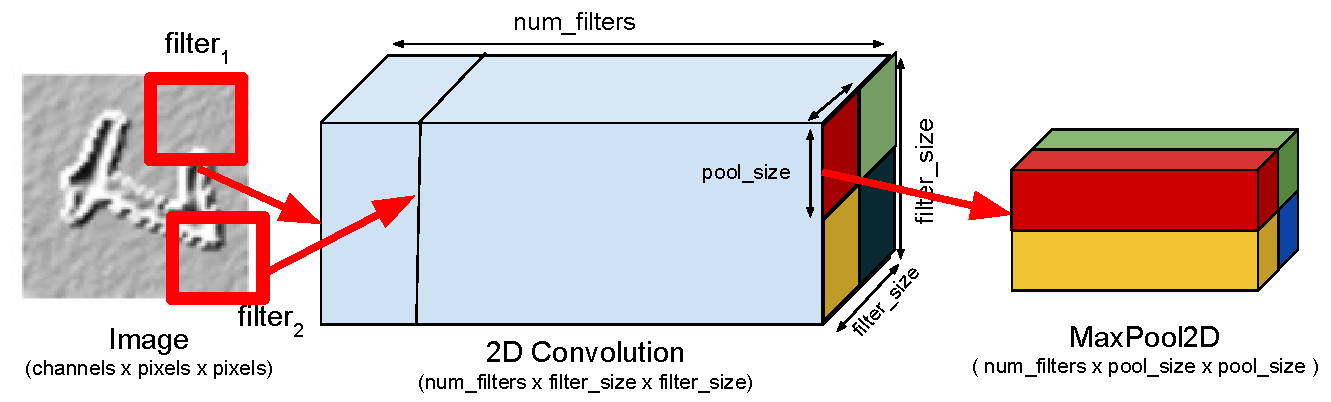
\includegraphics[scale=0.30]{convnet_example.pdf}
	\caption{A simplified example of the sublayer containing Convolution2D layer and a MaxPool2D layer. The variables correspond to the authors implementation of the network. The final network used one,two and three of these sublayers in tandem.}
	\label{convmaxlayer}
\end{figure}


\begin{figure}[h]
	% \centering
	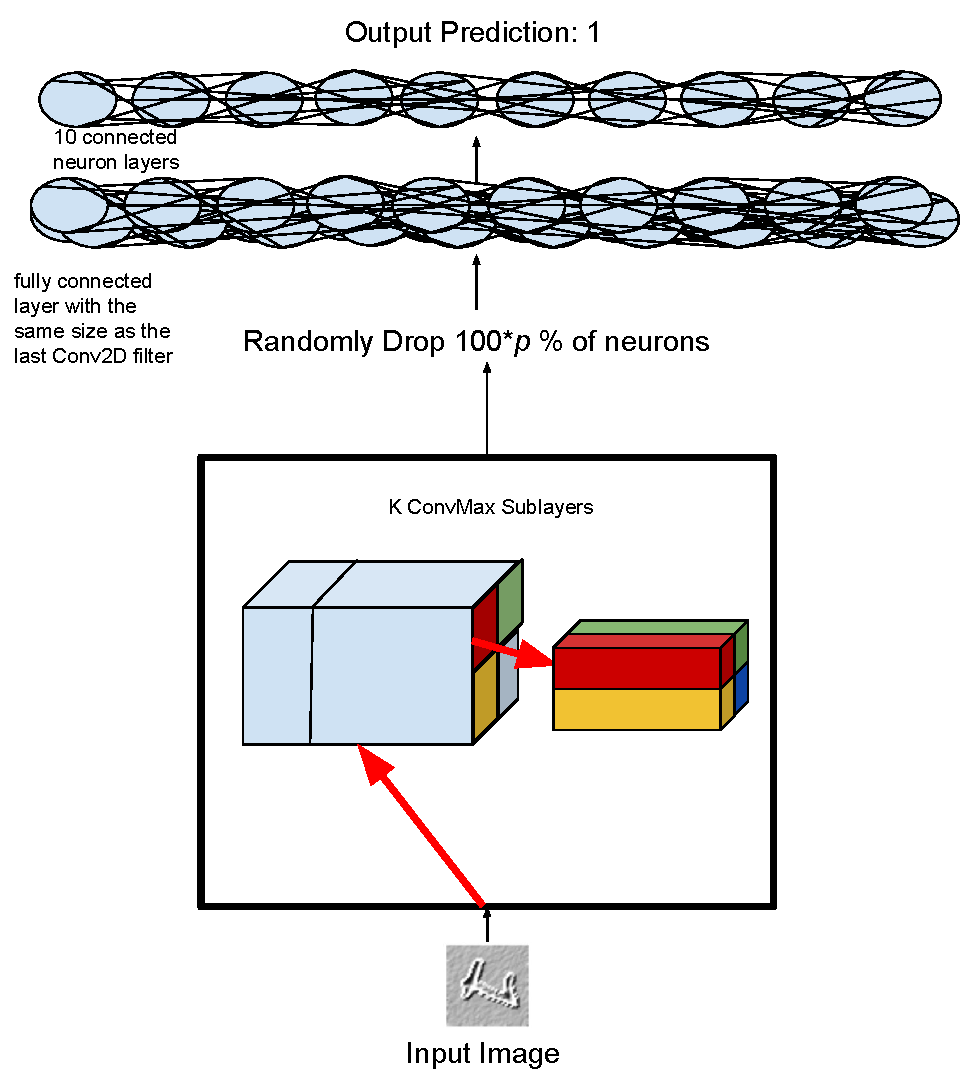
\includegraphics[scale=0.30]{architecture.pdf}
	\caption{The Convolution Neural Architechture included $k$ stacked sublayers shown in Fig \ref{convmaxlayer} connected to a dropout layer and finally fed into a fully connected layer containing $10$ neurons that did the final classification.}
	\label{CNNarch}
\end{figure}

\subsubsection{Spatial Transformer Network}

\subsection{Cross-Validation and Choice of Hyperparameters}

\section{Results}
\subsection{SVM}
Our grid search returned optimal values of C=10 and gamma=1e-4. We also cross validated several different kernels all with C=1 and a default gamma. RBF scored highest with about 32\% accuracy, next was a linear kernel with accuracy of about 29\%. Surprisingly all of the polynomial kernels performed as poorly as a random estimator (~10\% accuracy). This is surprising given the performance of the degree 9 SVM in \cite{LeCunn98}. A possible reason for this poor performance is that in order to speed up learning the number of iterations was set at a limit of 300. However, this same set up was used for the linear and RBF kernels as well and much better results were obtained with those methods. Further tests of an polynomial SVM without limiting the number of iterations also yielded the same poor results. The other explanation could be that in order to reduce train times and memory usage, only the first 30000 examples were used, and then a 64, 16, 20 split occurred for train, validate, test. The lack of training examples mixed with the fixed value of C (we did not perform grid search on C or gamma when picking a kernel) could have caused overfitting which would have caused the model to not generalize well. \ref{SVMGrid} shows a heat map of the search for a proper C and gamma. 

\begin{figure}[h]
	\centering
	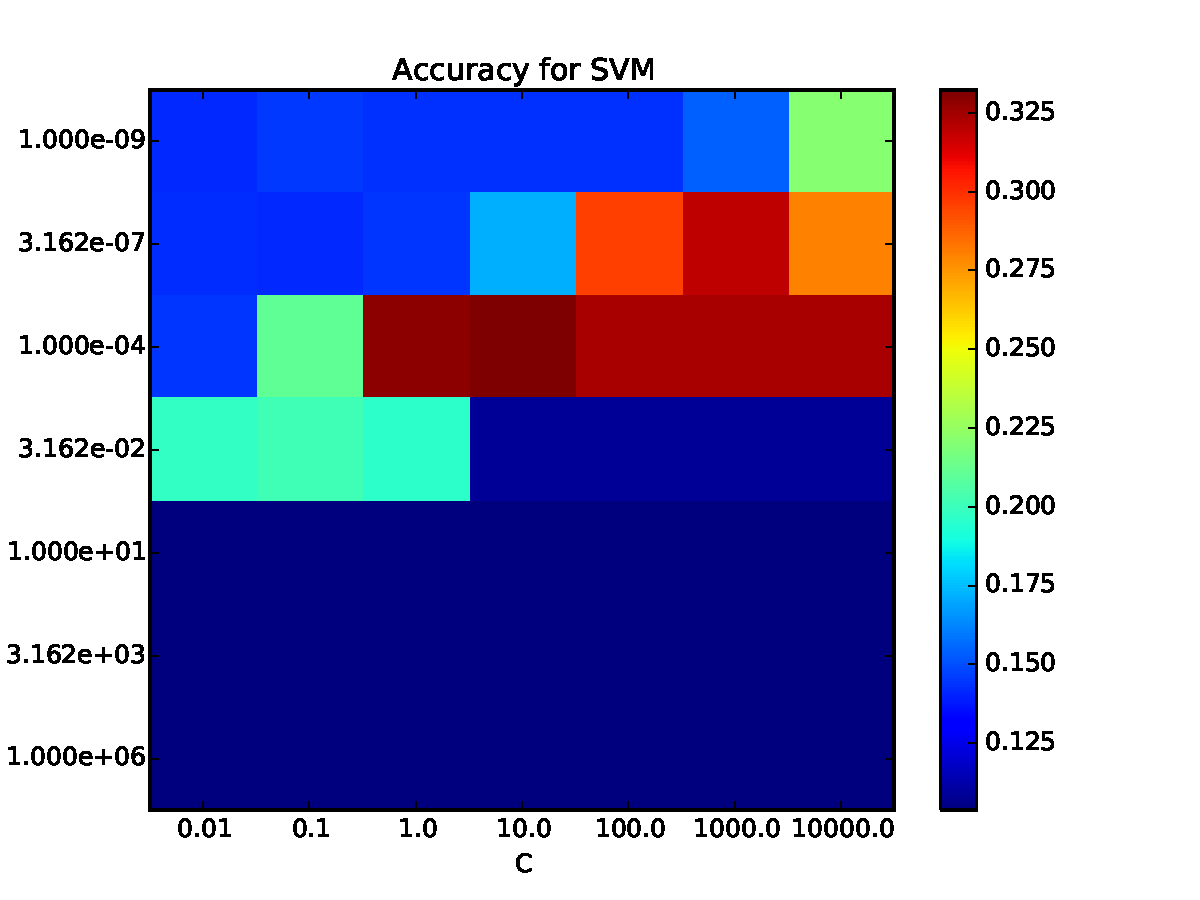
\includegraphics[scale=0.4]{SVM_grid_search.pdf}
	\caption{Heat map of SVM grid search}
	\label{SVMGrid}
\end{figure}
\subsection{Convolution Neural Network}
ROC (?) curves are shown in \label{CNN-ROC}

\begin{figure}[h]
	\centering
	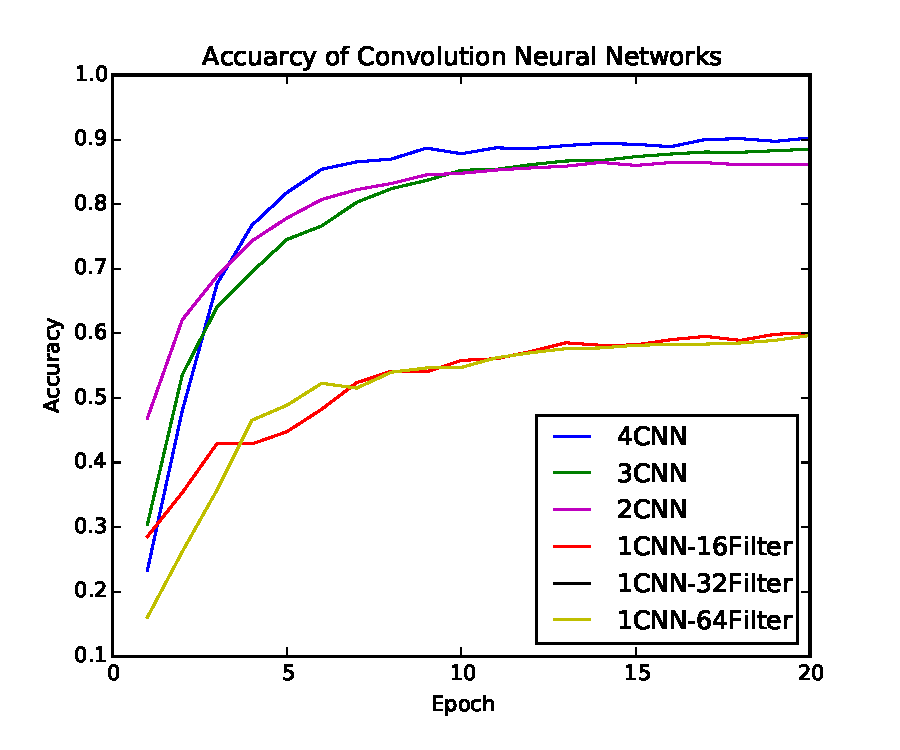
\includegraphics[scale=0.6]{CNNacc.pdf}
	\caption{ROC Curves for our CNN architectures}
	\label{CNN-ROC}
\end{figure}


\subsection{Spatial Transformer Network}



\section{Discussion}

\subsection{Feature Extraction and Selection}



\subsection{Classifier Performance}

\subsection{Future Work}



\section{Statement of Contributions}

\section{Integrity of work}
We hereby state that all the work presented in this report is that of the authors.
\begin{thebibliography}{9}

\bibitem{LeCunn98}
Lecun Y., Bengio Y., and Haffner P.
 \emph{Gradient-Based Learning Applied to Document Recognition}
 Proceedings of the IEEE,
 1998.

\bibitem{MNIST_Original}
Lecun Y., Cortes C. Burges C.
\emph{The MNIST database of handwritten digits} 
 
\bibitem{ML_textcat}
 Sebastini, F.
  \emph{Machine Learning in Automated Text Categorization}
  ACM Computing Surveys (CSUR) 34
  2002.

\bibitem{Hastie}
 Hastie T., Tibshirani R. Friedman J.
 \emph{The Elements of 
Statistical Learning: Data Mining, Inference, and Prediction}.
2nd edition
2009


\bibitem{CNN_committees}
 Claudiu D. and Meier U. et al.
  \emph{Convolutional Neural Network Committees For Handwritten Character
Classification}
  ACM Computing Surveys (CSUR) 34
  2002.

\bibitem{STN}
 Jaderberg, M., et al.
  \emph{Spatial Transformer Networks}
  ArXiv
  2015
  
\bibitem{Simard}
  Simard F., Steinkraus D., Platt J.
  \emph{Best Practices for Convolutional Neural Networks
Applied to Visual Document Analysis}
	Microsoft
    http://research.microsoft.com/pubs/68920/icdar03.pdf.

\bibitem{MnistHome}
LeCun Y., Cortes, C. and Burges C.J.C.
	\emph{The MNIST Database of handwritten digits}
	http://yann.lecun.com/exdb/mnist/
% inspiration for graphic http://cs231n.github.io/convolutional-networks/

\bibitem{sklearn}
Pedregosa F., Varoquaux G., Gramfort A., et al.
\emph{Scikit-learn: Machine Learning in {P}ython}
Journal of Machine Learning Research    
Vol 12, 2825-2830 2011   
       

\end{thebibliography}

\end{document}
